

\documentclass[10pt,conference]{IEEEtran}




% *** CITATION PACKAGES ***
%
\usepackage{cite}
\usepackage[cmex10]{amsmath}

\interdisplaylinepenalty=2500

\usepackage{amsthm}


% *** SPECIALIZED LIST PACKAGES ***
%
\usepackage{algorithmic}
\usepackage{array}
\usepackage{url}
\usepackage{xcolor}
\usepackage{epsfig}
\usepackage{subfig}

\newcommand{\exFigSize}{0.12}

\newcommand{\jef}[1]{\textcolor[rgb]{1,0,0}{[#1]}}


\begin{document}

\title{Technical Report: Exploiting Deep-Features Diversity in \jef{Dataset Type} Classification}

\author{\IEEEauthorblockN{Michael Jordan\IEEEauthorrefmark{1},
Homer Simpson\IEEEauthorrefmark{2},
Edson A. Nascimento\IEEEauthorrefmark{3}, 
Michael Jackson\IEEEauthorrefmark{3} and
Lewis Hamilton\IEEEauthorrefmark{4}}
\IEEEauthorblockA{\IEEEauthorrefmark{1}School of Electrical and Computer Engineering\\
Georgia Institute of Technology,
Atlanta, Georgia 30332--0250\\ Email: see http://www.michaelshell.org/contact.html}
\IEEEauthorblockA{\IEEEauthorrefmark{2}Twentieth Century Fox, Springfield, USA\\
Email: homer@thesimpsons.com}
\IEEEauthorblockA{\IEEEauthorrefmark{3}Starfleet Academy, San Francisco, California 96678-2391\\
Telephone: (800) 555--1212, Fax: (888) 555--1212}
\IEEEauthorblockA{\IEEEauthorrefmark{4}Tyrell Inc., 123 Replicant Street, Los Angeles, California 90210--4321}}

% make the title area
\maketitle

% As a general rule, do not put math, special symbols or citations
% in the abstract
%\begin{abstract}
%The abstract goes here.
%\end{abstract}

% no keywords




% For peerreview papers, this IEEEtran command inserts a page break and
% creates the second title. It will be ignored for other modes.
\IEEEpeerreviewmaketitle



\section{Introduction}

\jef{Include a brief description of the problem addressed by the chosen dataset. Include a brief explanation of the importance of your research regarding image classification
\vspace{13cm}.}

\section{Experimental Setup}

\subsection{Dataset}

\jef{Describe the dataset in details. Do not forget to include information on number of samples and number of classes. It is also interesting to include some sample images.\vspace{6cm}.}

\subsection{Implementation details}

\jef{Frameworks, Machine configuration, etc.\vspace{6cm}.}

\section{Results and Discussion}

\subsection{Deep features comparison}

\jef{Comment on Figure~\ref{fig:feat_comp}.\vspace{3cm}}

\begin{figure*}[h!]
	\centering
	\scriptsize
	\subfloat[$C1$]{
		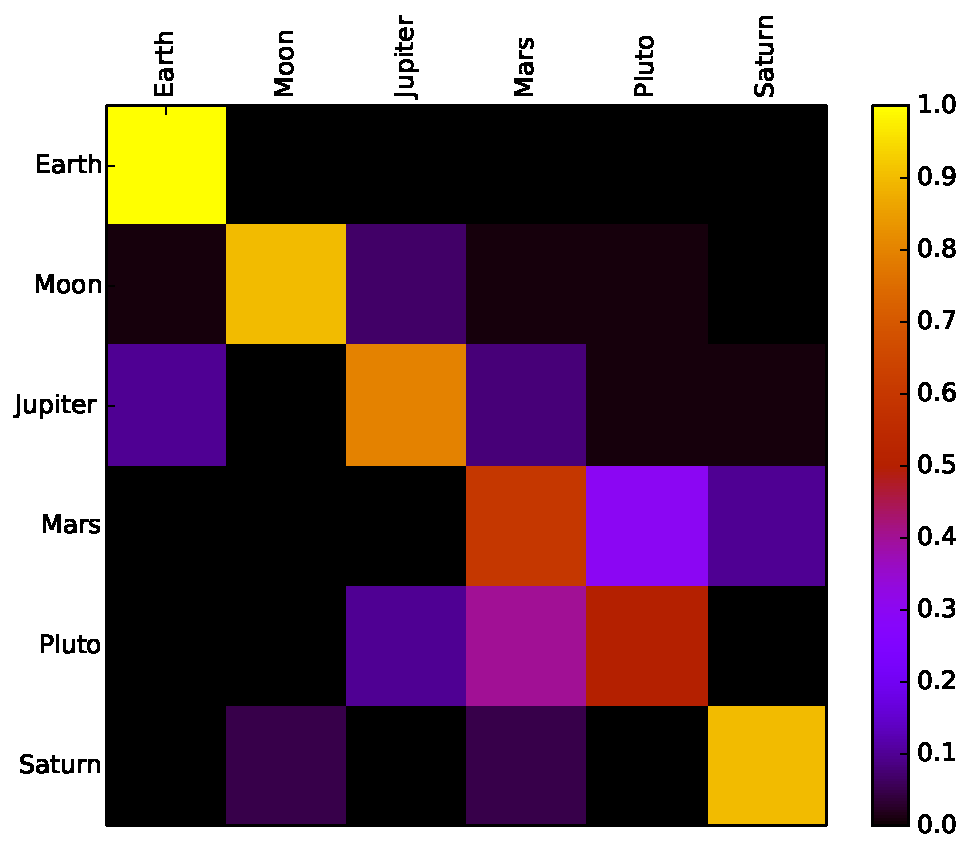
\includegraphics[width=0.30\textwidth, keepaspectratio=true]{figs/heatmap_example.pdf}
	}
	\hspace{1mm}
	\subfloat[$C5$]{
		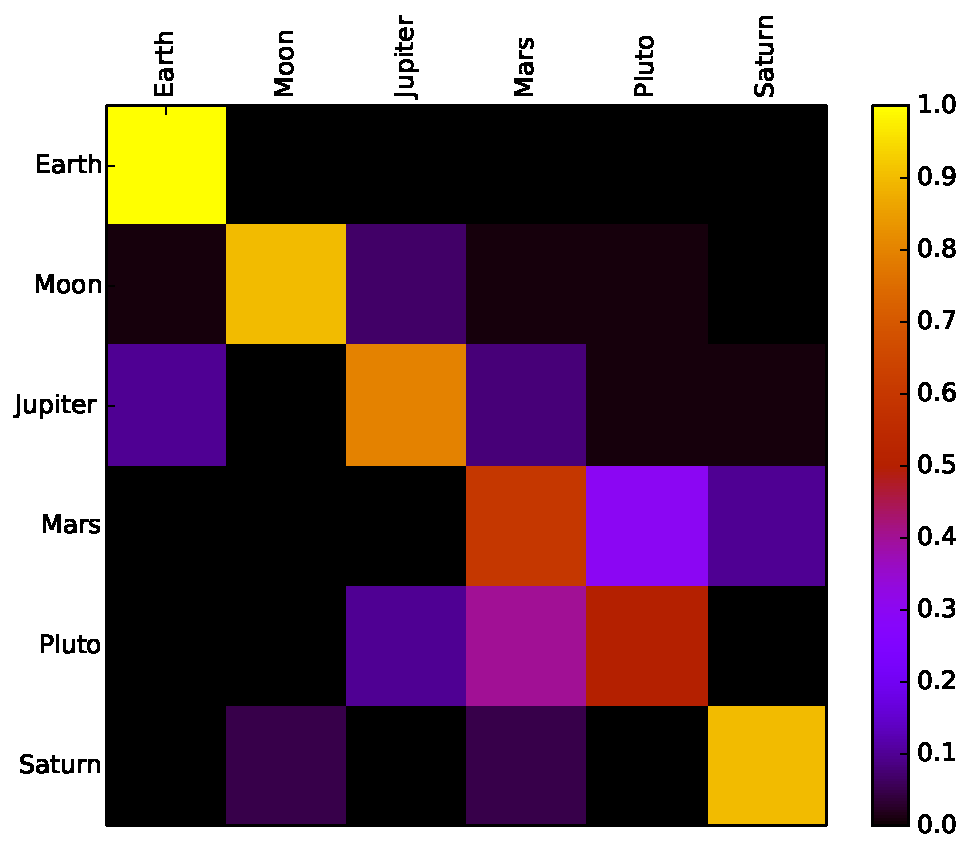
\includegraphics[width=0.30\textwidth, keepaspectratio=true]{figs/heatmap_example.pdf}
	}
	\hspace{1mm}
	\subfloat[$FC2$]{
		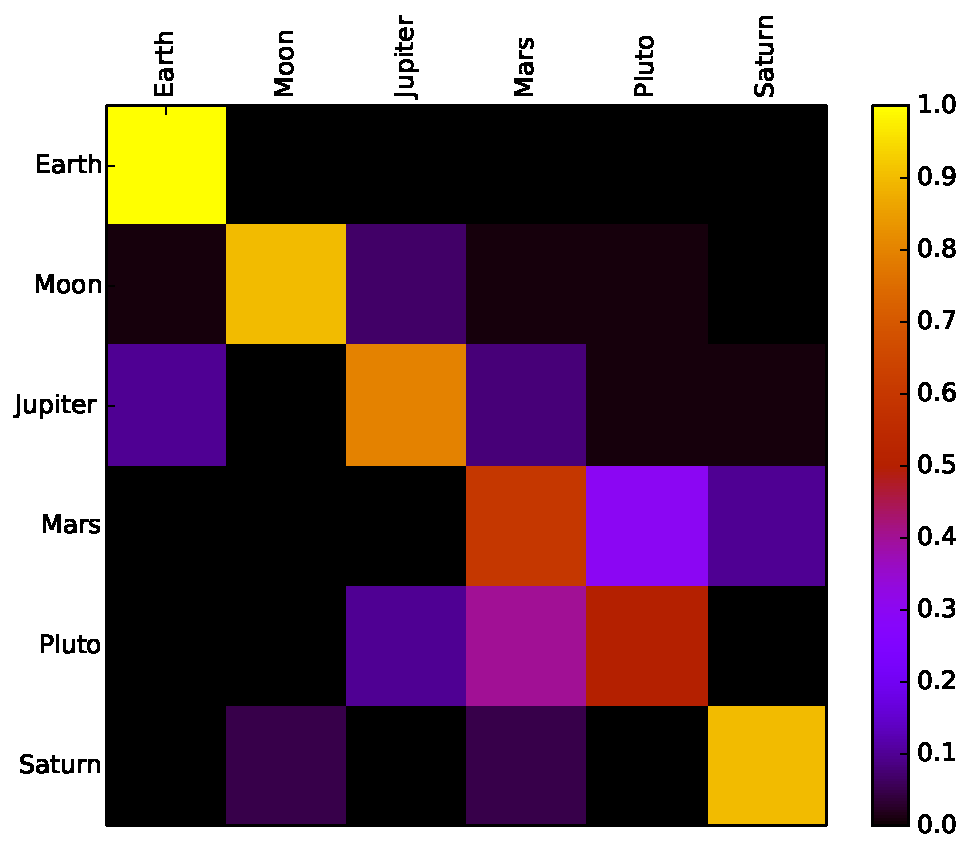
\includegraphics[width=0.30\textwidth, keepaspectratio=true]{figs/heatmap_example.pdf}
	}
	\caption{Classification results for each class by using SVM-RBF with features $C1$, $C5$, and $FC2$, respectively.}
	\label{fig:feat_comp}
\end{figure*}

\jef{Comment on Table~\ref{tab:feat_comp}.\vspace{3cm}}

\begin{table}[h!]
	\caption{Classification results with different deep representation levels.}
	\label{tab:feat_comp}
	\center{
		\begin{tabular}{lcc} \hline
			\textbf{Approach}		& \textbf{O.A. (\%)}	& \textbf{A.A. (\%)}	\\ \hline 
			\emph{$C1$}		& $00.00 \pm 00.00$ 	& $00.00 \pm 00.00$\\
			\emph{$C5$}		& $00.00 \pm 00.00$	& $00.00 \pm 00.00$\\
			\emph{$FC2$}		& $00.00 \pm 00.00$	& $00.00 \pm 00.00$\\
			\hline 
		\end{tabular}
	}
\end{table}


\subsection{Deep features combination}

\jef{Comment on Figure~\ref{fig:feat_comb}.\vspace{3cm}}

\begin{figure*}[ht!]
	\centering
	\scriptsize
	\subfloat[Early fusion]{
		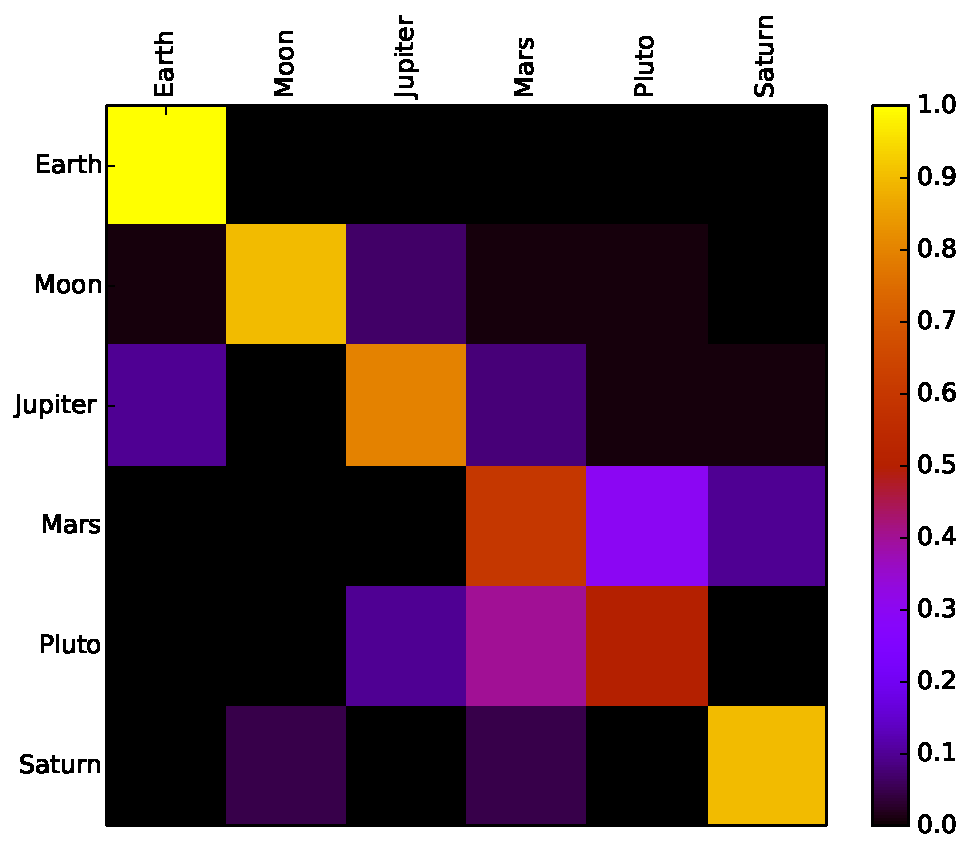
\includegraphics[width=0.30\textwidth, keepaspectratio=true]{figs/heatmap_example.pdf}
	}
	\hspace{1mm}
	\subfloat[Late fusion]{
		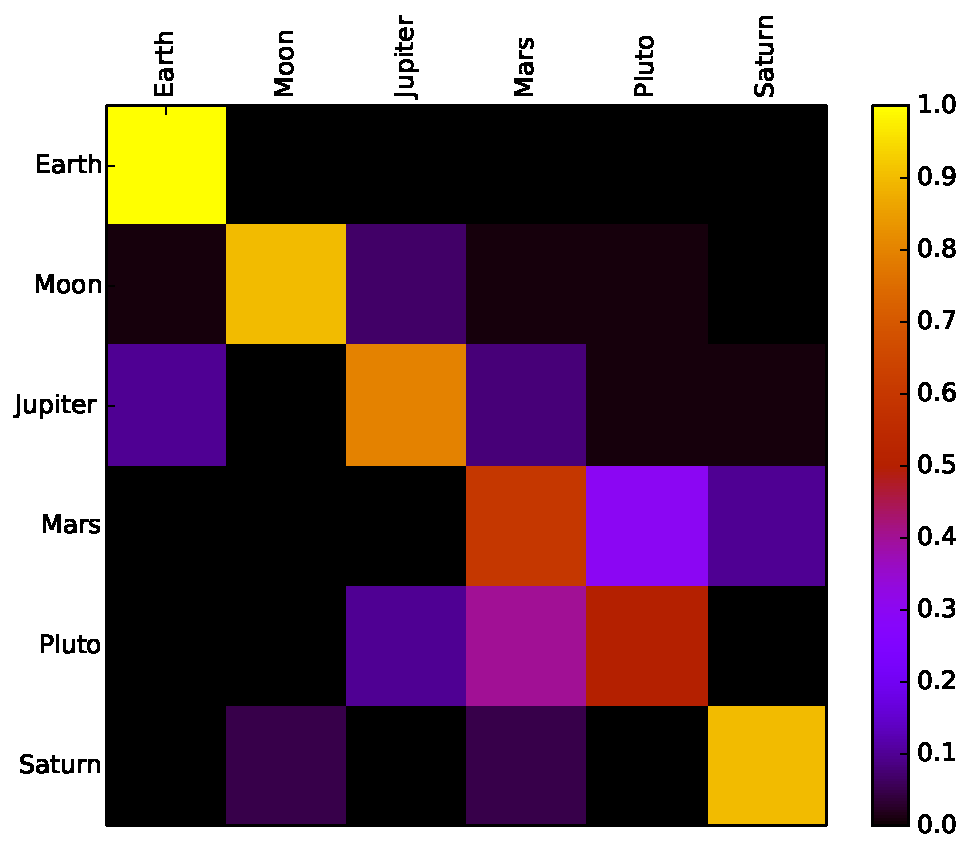
\includegraphics[width=0.30\textwidth, keepaspectratio=true]{figs/heatmap_example.pdf}
	}
	\hspace{1mm}
	\subfloat[\jef{best feature}]{
		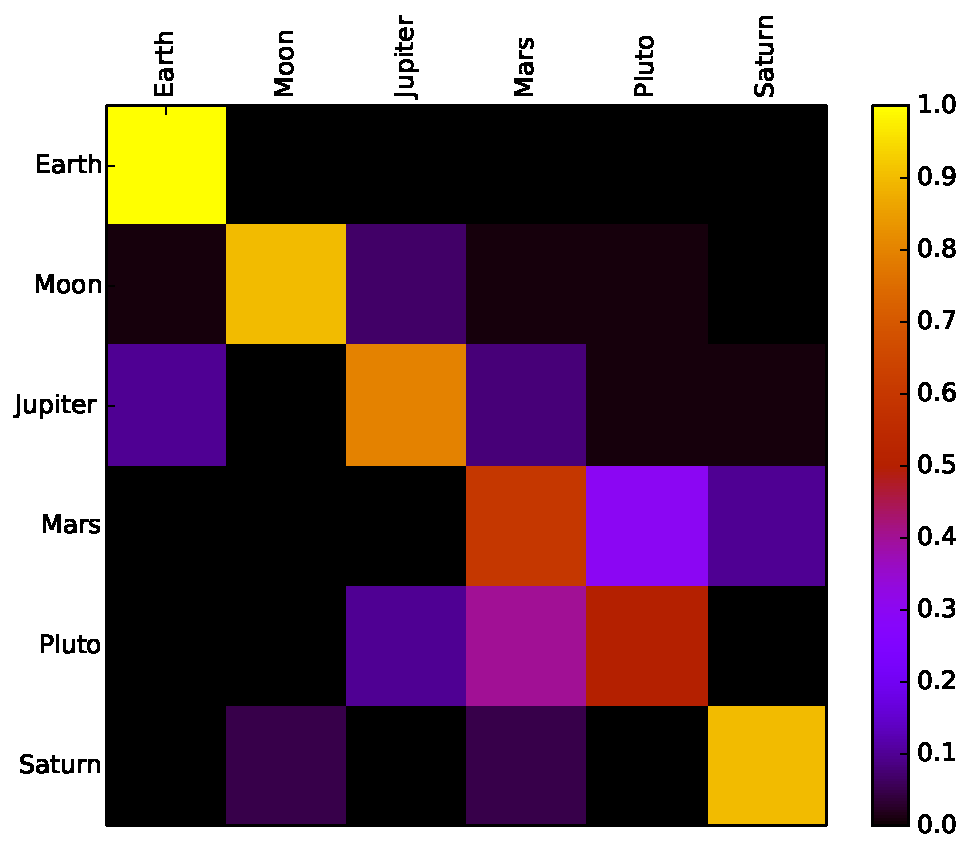
\includegraphics[width=0.30\textwidth, keepaspectratio=true]{figs/heatmap_example.pdf}
	}
	\caption{Classification results for each class by using early fusion, late fusion, and \jef{best feature}.}
	\label{fig:feat_comb}
\end{figure*}

\jef{Comment on Table~\ref{tab:feat_comb}.\vspace{3cm}}

\begin{table}[ht!]
	\caption{Classification results by using early fusion, late fusion, and \jef{best feature}.}
	\label{tab:feat_comb}
	\center{
		\begin{tabular}{lcc} \hline
			\textbf{Approach}		& \textbf{O.A. (\%)}	& \textbf{A.A. (\%)}	\\ \hline 
			\emph{Early fusion}		& $00.00 \pm 00.00$ 	& $00.00 \pm 00.00$\\
			\emph{Late fusion}		& $00.00 \pm 00.00$	& $00.00 \pm 00.00$\\
			\emph{\jef{best feature}}		& $00.00 \pm 00.00$	& $00.00 \pm 00.00$\\
			\hline 
		\end{tabular}
	}
\end{table}

\subsection{Diversity evaluation}

\jef{Comment on Figure~\ref{fig:diversity}.\vspace{4cm}}

\begin{figure*}[ht!]
	\centering
	\scriptsize
	\subfloat[Random Forest]{
		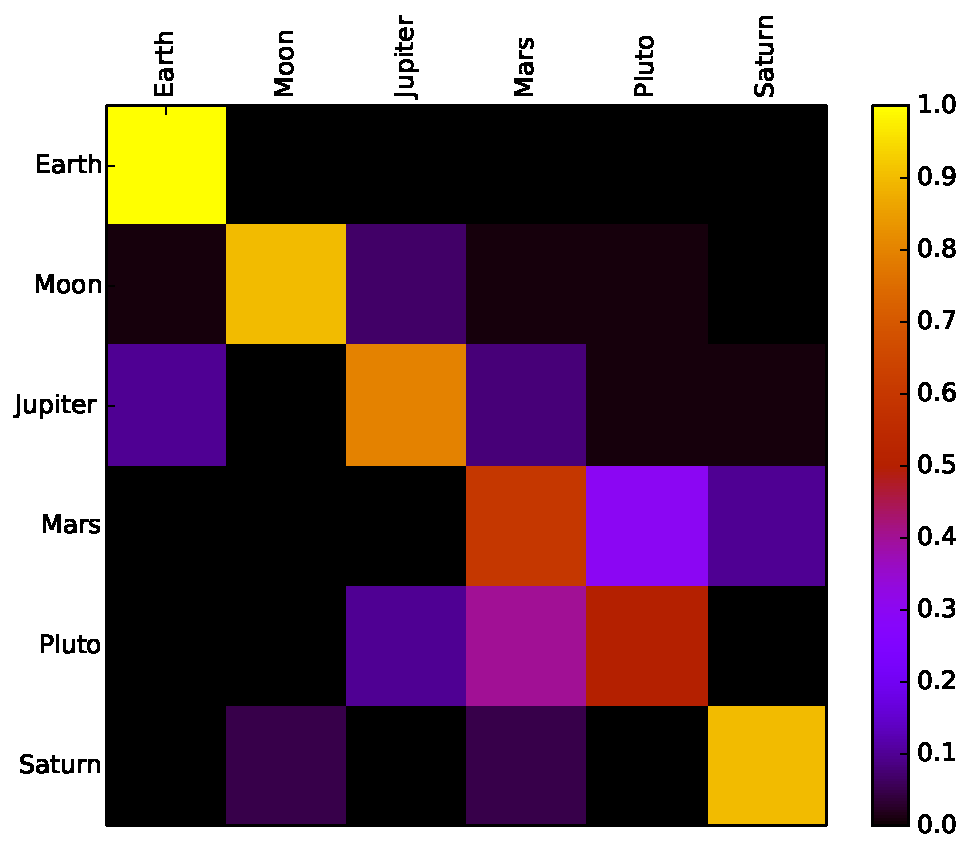
\includegraphics[width=0.30\textwidth, keepaspectratio=true]{figs/heatmap_example.pdf}
	}
	\hspace{1mm}
	\subfloat[Majority Voting]{
		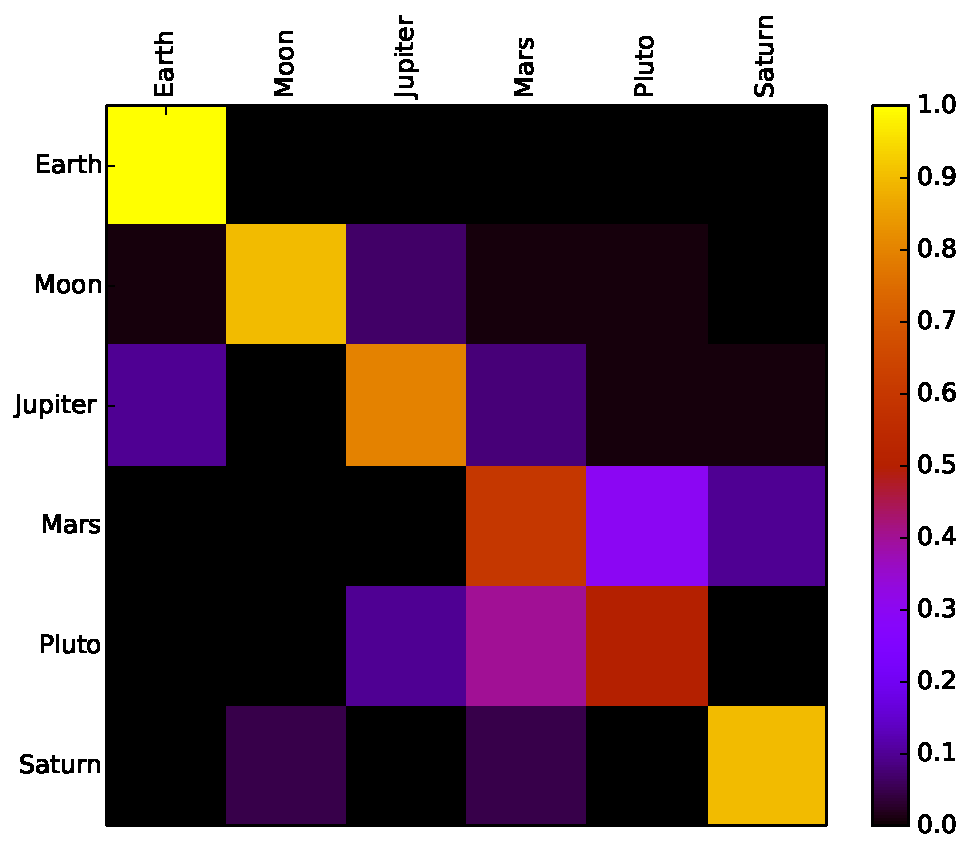
\includegraphics[width=0.30\textwidth, keepaspectratio=true]{figs/heatmap_example.pdf}
	}
	\hspace{1mm}
	\subfloat[Bagging]{
		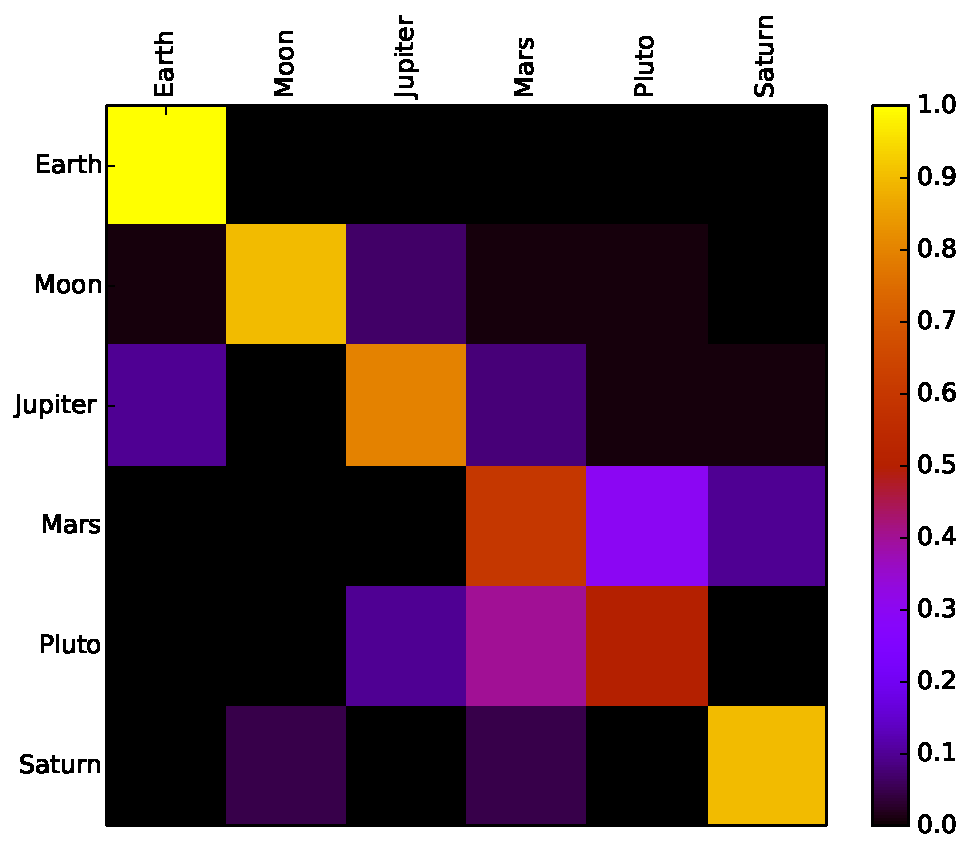
\includegraphics[width=0.30\textwidth, keepaspectratio=true]{figs/heatmap_example.pdf}
	}
	\caption{Classification results for each class by using ensemble approaches.}
	\label{fig:diversity}
\end{figure*}

\jef{Comment on Table~\ref{tab:diversity}.\vspace{3cm}}

\begin{table}[h!]
	\caption{Classification results by using ensemble methods in comparison with original deep features.}
	\label{tab:diversity}
	\center{
		\begin{tabular}{lcc} \hline
			\textbf{Approach}		& \textbf{O.A. (\%)}	& \textbf{A.A. (\%)}	\\ \hline 
			\emph{SVM-RBF ($FC2$)}		& $00.00 \pm 00.00$	& $00.00 \pm 00.00$\\
			\emph{Random Forest}		& $00.00 \pm 00.00$ 	& $00.00 \pm 00.00$\\
			\emph{Majority Voting}		& $00.00 \pm 00.00$	& $00.00 \pm 00.00$\\
			\emph{Bagging}		& $00.00 \pm 00.00$	& $00.00 \pm 00.00$\\			
			\hline 
		\end{tabular}
	}
\end{table}

\section{Conclusions}

\jef{The conclusion goes here.\vspace{7cm}}




% conference papers do not normally have an appendix


% use section* for acknowledgment
\section*{Acknowledgment}


The authors would like to thank...


% trigger a \newpage just before the given reference
% number - used to balance the columns on the last page
% adjust value as needed - may need to be readjusted if
% the document is modified later
%\IEEEtriggeratref{8}
% The "triggered" command can be changed if desired:
%\IEEEtriggercmd{\enlargethispage{-5in}}

% references section

% can use a bibliography generated by BibTeX as a .bbl file
% BibTeX documentation can be easily obtained at:
% http://mirror.ctan.org/biblio/bibtex/contrib/doc/
% The IEEEtran BibTeX style support page is at:
% http://www.michaelshell.org/tex/ieeetran/bibtex/
\bibliographystyle{IEEEtran}
% argument is your BibTeX string definitions and bibliography database(s)
\bibliography{example}
%
% <OR> manually copy in the resultant .bbl file
% set second argument of \begin to the number of references
% (used to reserve space for the reference number labels box)
%\begin{thebibliography}{1}
%
%\bibitem{IEEEhowto:kopka}
%H.~Kopka and P.~W. Daly, \emph{A Guide to \LaTeX}, 3rd~ed.\hskip 1em plus
%  0.5em minus 0.4em\relax Harlow, England: Addison-Wesley, 1999.

%\end{thebibliography}




% that's all folks
\end{document}


